% !TEX root = thesis.tex
\documentclass[12pt,a4paper,titlepage,listof=totoc,bibliography=totoc,chapteratlists=0pt]{scrreprt}
\newcommand{\thesislang}{de} % en or de
\newcommand{\thesistitle}{Unser Thema ist Memoryland}
\newcommand{\department}{Informatik \& Medientechnik} % Replace with your department

\newcommand{\firstauthor}{Arwed Schnalzenberger, 5BHIF}
\newcommand{\secondauthor}{Isabel Schnalzenberger, 5AHITM}

\newcommand{\duedateen}{2025} % due date in English format
\newcommand{\duedatede}{2025} % due date in German format
\newcommand{\supervisor}{Prof. Christian Aberger}
\newcommand{\projectpartner}{Keine}
\begin{filecontents*}{\jobname.xmpdata}
	\Keywords{Angular,Azure,Picture,Unity}
	\Title{Memoryland}
	\Author{Arwed Schnalzenberger, Isabel Schnalzenberger}
\end{filecontents*}

\setcounter{tocdepth}{1}

\usepackage[utf8]{inputenc}
\usepackage[T1]{fontenc}
\usepackage{amsmath}
\usepackage{amsfonts}
\usepackage{amssymb}
\usepackage[table]{xcolor}
\usepackage{graphicx}
\usepackage[left=3.50cm, right=2.00cm, top=2.00cm, bottom=2.00cm,foot=1cm]{geometry}
\usepackage[splitrule,hang,flushmargin,multiple,bottom]{footmisc}
\usepackage{lmodern, textcomp}
\usepackage{lmodern}
\usepackage{pdfpages}
\usepackage[ngerman]{babel}
\usepackage{multicol}
\usepackage{float}
\usepackage{array,tabularx,booktabs}
\usepackage{ragged2e}
\usepackage{lipsum}
\usepackage{wrapfig}
\usepackage{xstring}
\usepackage{tocbasic}

\newcolumntype{M}[1]{>{\centering\arraybackslash}m{#1}}

\usepackage{enumitem}
\newlist{compactitem}{itemize}{3}
\setlist[compactitem,1]{label=\textbullet, nosep,leftmargin=1.5em,labelwidth=*,align=left}
\setlist[compactitem,2]{label=--, nosep,leftmargin=1.5em,labelwidth=*,align=left}
\setlist[compactitem,3]{label=\textopenbullet, nosep,leftmargin=1.5em,labelwidth=*,align=left}
\newlist{compactenum}{enumerate}{3}
\setlist[compactenum,1]{label=\arabic*., nosep,leftmargin=1.5em,labelwidth=*,align=left}
\setlist[compactenum,2]{label=\alph*., nosep,leftmargin=1.5em,labelwidth=*,align=left}
\setlist[compactenum,3]{label=\roman*., nosep,leftmargin=1.5em,labelwidth=*,align=left}
\newlist{compactdesc}{description}{3}
\setlist[compactdesc]{leftmargin=1.5em,labelwidth=*,align=left}

\usepackage{microtype}

\usepackage[parfill]{parskip}

\definecolor{bluekeywords}{rgb}{0.13,0.13,1}
\definecolor{greencomments}{rgb}{0,0.5,0}
\definecolor{redstrings}{rgb}{0.9,0,0}
\definecolor{lightgray}{gray}{0.9}
\definecolor{lightblue}{rgb}{0.93,0.95,1.0}

\usepackage{listings}

\makeatletter
\lstdefinestyle{lststyle}{
	basicstyle=%
	\ttfamily
	\lst@ifdisplaystyle\scriptsize\fi
}
\makeatother

\renewcommand{\lstlistlistingname}{List of Listings}
% TODO: define other languages as needed
\lstset{language=Python,
numbers=left,               
numberstyle=\tiny,          
showspaces=false,
showtabs=false,
breaklines=true,
lineskip=-1pt,
tabsize=2,
showstringspaces=false,
breakatwhitespace=true,
escapeinside={(*@}{@*)},
commentstyle=\color{greencomments},
keywordstyle=\color{bluekeywords}\bfseries,
stringstyle=\color{redstrings},
style=lststyle,
xleftmargin=17pt,
         framexleftmargin=17pt,
         framexrightmargin=5pt,
         framexbottommargin=4pt
}
\lstset{
morekeywords={base,var,in,out,dynamic,from,where,select,orderby,function,\$,group,by,into,yield,async,await,@,None,self,as,elif,with}
}
\lstdefinelanguage{TypeScript}{
	keywords={typeof, new, true, false, catch, function, return, null, switch, var, if, in, while, do, else, case, break, void, number, string, boolean, module, \$, export, for, this},
	keywordstyle=\color{blue}\bfseries,
	ndkeywords={class, export, boolean, throw, implements, import, this},
	ndkeywordstyle=\color{darkgray}\bfseries,
	identifierstyle=\color{black},
	sensitive=false,
	comment=[l]{//},
	morecomment=[s]{/*}{*/},
	commentstyle=\color{purple}\ttfamily,
	stringstyle=\color{red}\ttfamily,
	morestring=[b]',
	morestring=[b]"
}
\usepackage{caption}
\DeclareCaptionFont{white}{\color{white}}
\DeclareCaptionFormat{listing}{\colorbox[cmyk]{0.43, 0.35, 0.35,0.01}{\parbox{\textwidth}{\hspace{10pt}#1#2#3}}}
\captionsetup[lstlisting]{format=listing,labelfont=white,textfont=white} 
\captionsetup[table]{justification=centering, singlelinecheck=false}

\usepackage{subcaption}

\usepackage{setspace}
\newcommand{\MSonehalfspacing}{%
	\setstretch{1.44}%  default
	\ifcase \@ptsize \relax % 10pt
	\setstretch {1.448}%
	\or % 11pt
	\setstretch {1.399}%
	\or % 12pt
	\setstretch {1.433}%
	\fi
}

\newcommand{\setauthor}[1]{\ohead[]{#1}}

\usepackage[automark]{scrlayer-scrpage}
\pagestyle{scrheadings}
\automark{chapter}
\renewcommand\sectionmark[1]{\markright{\MakeMarkcase {\thesection\hskip .5em\relax#1}}}
\rohead{\ifnum\expandafter\pdfstrcmp\botmark=0 \rightmark\else\leftmark{} --- \rightmark\fi}
\ihead[]{\headmark}
\chead[]{}
\ohead{}
\cfoot[]{}
\ofoot[\pagemark]{\pagemark}
\setheadsepline{.1pt}

\usepackage[hyphens]{url}

\usepackage[a-1b]{pdfx}

\usepackage{hyperref}
\hypersetup{pdfa}

\usepackage[nonumberlist,toc,nopostdot]{glossaries}

\usepackage{chngcntr}
\counterwithout{footnote}{chapter}
\counterwithout{figure}{chapter}
\counterwithout{table}{chapter}
\AtBeginDocument{
	\counterwithout{lstlisting}{chapter}
	\urlstyle{sf}
}
\newcounter{RPages}

\makeatletter
\def\bstctlcite{\@ifnextchar[{\@bstctlcite}{\@bstctlcite[@auxout]}}
\def\@bstctlcite[#1]#2{\@bsphack
	\@for\@citeb:=#2\do{%
		\edef\@citeb{\expandafter\@firstofone\@citeb}%
		\if@filesw\immediate\write\csname #1\endcsname{\string\citation{\@citeb}}\fi}%
	\@esphack}
\makeatother

\clubpenalty=10000 
\widowpenalty=10000
\displaywidowpenalty=10000
\interfootnotelinepenalty=10000

\title{\thesistitle}
\makeatletter
\@ifundefined{fourthauthor}{
  \@ifundefined{thirdauthor}{
    \author{\firstauthor, \secondauthor}
  }{
    \author{\firstauthor, \secondauthor, \thirdauthor}
  }
}{
  \author{\firstauthor, \secondauthor, \thirdauthor, \fourthauthor}
}
\makeatother

\makeindex
\makeglossaries
\begin{document}
\bstctlcite{IEEEexample:BSTcontrol}
\newcommand{\reminder}[1]
{ \textcolor{red}{<[{\bf\marginpar{\mbox{$<==$}} #1 }]>} }
\newcommand{\icode}[1]{\lstinline$#1$}
%\urlstyle{same}
%\setstretch{1.5}
\setstretch {1.433}
\renewcommand{\arraystretch}{1.2}

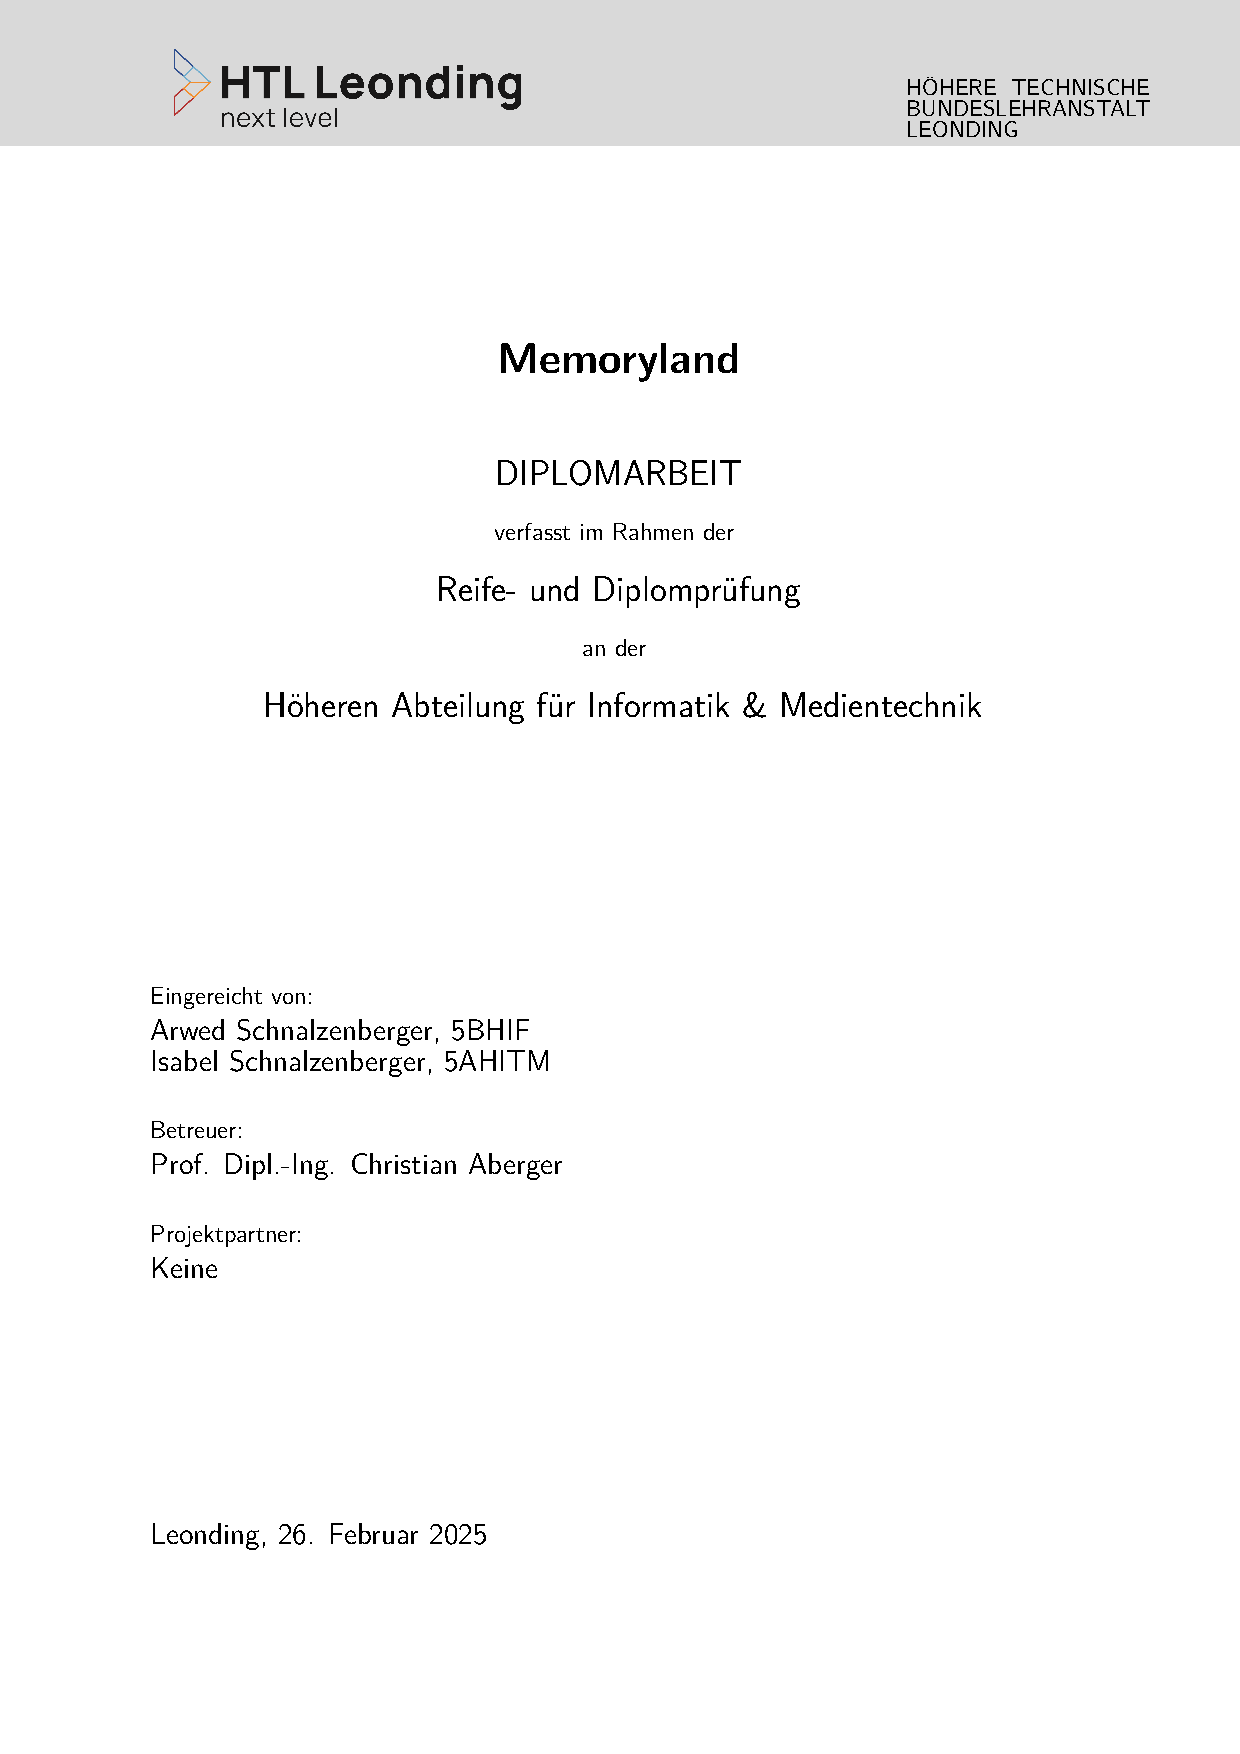
\includepdf{./titlepage/coversheet}
\pagenumbering{Roman}
\newpage
\thispagestyle{empty}
\vspace{3cm}
~ \\ \\
\IfStrEq{\thesislang}{de}
{
Ich erkläre an Eides statt, dass ich die vorliegende Diplomarbeit selbstständig und ohne fremde Hilfe verfasst, andere als die angegebenen Quellen und Hilfsmittel nicht benutzt bzw. die wörtlich oder sinngemäß entnommenen Stellen als solche kenntlich gemacht habe.

Die Arbeit wurde bisher in gleicher oder ähnlicher Weise keiner anderen Prüfungsbehörde vorgelegt und auch noch nicht veröffentlicht.

Die vorliegende Diplomarbeit ist mit dem elektronisch übermittelten Textdokument identisch.
}
{
I hereby declare that I have composed the presented paper independently and on my own, without any other resources than the ones indicated. 
All thoughts taken directly or indirectly from external sources are properly denoted as such.

This paper has neither been previously submitted to another authority nor has it been published yet.

The presented paper is identical to the electronically transmitted document.
}
\vspace{3cm}
% Hier kommt die Unterschrift drüber
\begin{tabbing}
Leonding, \IfStrEq{\thesislang}{de}{\duedatede}{\duedateen} \hspace{2cm} {\firstauthor} \& {\secondauthor} %, \thirdauthor \& \fourthauthor % replace & with , for all but the last author
\end{tabbing}
\vspace{10cm}
\newpage
\setcounter{page}{1}

\begin{spacing}{1}
    \chapter*{Abstract}
\end{spacing}
\begin{wrapfigure}{r}{0.3\textwidth}
    \begin{center}
      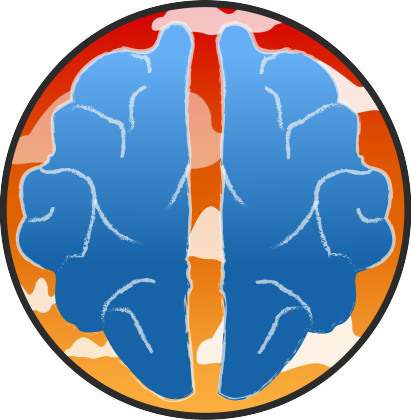
\includegraphics[width=0.2\textwidth]{pics/memoryland-logo.png}
    \end{center}
\end{wrapfigure}

Memories in the form of photos and videos are a valuable part of life, yet they are often 
lost or rarely revisited. To keep these memories alive, an appealing presentation and easy 
accessibility are essential.

The diploma project Memoryland was developed to address exactly this issue. It allows 
personal memories to be experienced in an interactive and animated form and to share them with 
others. As part of this project, a web application was created that transforms photos into 
engaging animations. Users can generate videos from these animations and share them with 
their friends.

A special focus was placed on creating an immersive experience. Memorylands enable 
users to relive their memories in virtual environments such as a forest or an island. 
Additionally, great care was taken to ensure that the functionalities are as intuitive
and comfortable as possible.

Ultimately, this project aims to make it easier for people to preserve their memories 
in a creative and entertaining way while allowing them to rediscover them effortlessly.

\newpage
\begin{spacing}{1}
    \chapter*{Zusammenfassung}
\end{spacing}
\begin{wrapfigure}{r}{0.3\textwidth}
    \begin{center}
      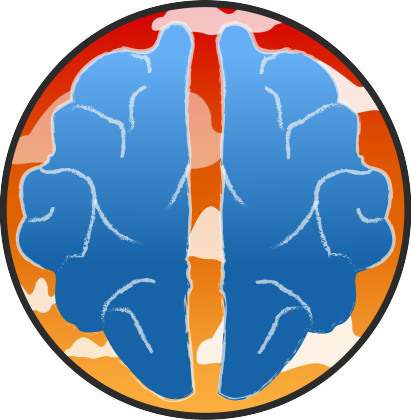
\includegraphics[width=0.2\textwidth]{pics/memoryland-logo.png}
    \end{center}
\end{wrapfigure}
Erinnerungen in Form von Fotos und Videos sind ein wertvoller Bestandteil des Lebens und doch
gehen sie oft verloren oder werden selten angesehen. Um diese Erinnerungen lebendig zu halten,
sind daher eine ansprechende Präsentation und einfache Zugänglichkeit essenziell.

Die Diplomarbeit Memoryland wurde entwickelt, um genau dieses Problem zu lösen. Sie ermöglicht es, 
persönliche Erinnerungen in einer interaktiven und animierten Form zu erleben und mit anderen zu 
teilen. Im Rahmen dieser Arbeit wurde eine Web-Anwendung erstellt, die Fotos in ansprechende 
Animationen umwandelt. Daraus können Nutzer:innen nun Videos generieren und an ihre Freunde 
weitergeben.

Besonderes wurde hierbei auf eine immersive Erfahrung geachtet. Memorylands ermöglichen es, 
Erinnerungen in einer virtuellen Umgebung, wie einem Wald oder einer Insel, zu erleben. Es
wurde auch darauf geachtet, dass die Funktionalitäten so intuitiv und gemütlich wie möglich
sind.

Schlussendlich soll unsere Arbeit es Menschen erleichtern, ihre Erinnerungen auf eine 
kreative und unterhaltsame Weise zu wahren und leicht wiederzuentdecken.



\pagestyle{plain}

\IfStrEq{\thesislang}{de}
{
	\renewcommand{\lstlistlistingname}{Quellcodeverzeichnis}
}
{
 % keep at list of listing
}

\tableofcontents
\newpage
\setcounter{RPages}{\value{page}}
\setcounter{page}{0}
\pagenumbering{arabic}
\pagestyle{scrheadings}

\begin{spacing}{1}
\chapter{Einleitung}\label{chapter:introduction}
\end{spacing}

\section{Ursprüngliche Idee}

\section{Ausgangssituation}

Herkömmliche Familien-/Fotoalben stehen normalerweise wegen ihres Gewichtes 
zuhause und falls man dann einmal einem Freund bei einer Party ein Foto schnell 
zeigen möchte, hat man eher das Handy als ein ganzes Fotoalbum dabei.
\\
Zwar gibt es schon Tools, welche die Fotos nur präsentieren, 
aber wir wollen die Fotos zeitgemäß für jeden leicht verfügbar und transportabel animieren.

\section{Untersuchungsanliegen}

Arwed Schnalzenberger:
\begin{itemize}
\item Die vorliegende Untersuchung zielt darauf ab, die effiziente Speicherung 
umfangreicher Mengen von Videos und Bildmaterial in Cloud-Umgebungen zu 
untersuchen sowie die Prozesse zur Erstellung und Bearbeitung von Videos 
auf der Backend-Ebene zu erforschen.
\end{itemize}


Isabel Schnalzenberger:
\begin{itemize}
\item Die vorliegende Untersuchung zielt darauf ab, die potenzielle Steigerung 
der Akzeptanz von Online-Darstellungen durch die Integration von 
3D-Visualisierungen einer Bildergalerie zu erforschen.
\end{itemize}

\begin{spacing}{1}
\chapter{Umfeldanalyse}
\end{spacing}
Bereits vor der Entwicklung von Memoryland, gab es bestehende Lösungen zur Verwaltung
und Präsentation von Erinnerungen. Bevor mit dem Projekt begonnen wurde, wurden
diese analysiert und die Erkenntnisse zu den Stärken und Schwächen dieser Systeme
notiert. Daraus entstanden dann die Anforderungen für das finale System.

\section{Analyse der vorhandenen Systeme}

\subsection{OneDrive}

\emph{Vorteile:}
Das System bietet eine cloudbasierte Speicherung für Bilder und andere Medien. 
So können Nutzer:innen ihre Dateien zentral ablegen und von verschiedenen Geräten aus darauf 
zugreifen.

\emph{Nachteile:}
Eine Integration von Bildern in interaktive Formate ist nicht vorhanden. 
Dadurch bleibt die Nutzung der gespeicherten Bilder auf eine einfache 
Anzeige und Verwaltung beschränkt.

\emph{Zusammenfassung:}
OneDrive bietet eine sichere und cloudbasierte Speicherung von Bildern und anderen 
Medien. Es fehlen Funktionen zur Bildbearbeitung und zur Integration von 
immersiven Formaten. \footnote{Informationen zu OneDrive stammen von \cite{MicrosoftCorporation}}

\subsection{Google Photos}

\emph{Vorteile:}
Das System stellt eine Oberfläche für eine Verwaltung und Anzeige von Bildern 
zur Verfügung. Dadurch können Nutzer:innen ihre Bilder organisieren und betrachten.

\emph{Nachteile:}
Eine Integration von Bildern in interaktive Formate ist nicht vorhanden. 
Somit ist es nicht möglich sie in erweiterte Präsentationsformen einzubinden 
und beschränkt die Nutzung der Bilder auf Verwaltungs- und Anzeigezwecke.

\emph{Zusammenfassung:}
Google Photos ermöglicht eine Verwaltung und Anzeige von Bildern, bietet jedoch 
keine Möglichkeit zur Umwandlung von Bildern in interaktive Formate. \footnote{Informationen zu Google Photos stammen von \cite{GoogleIrelandLimited}}

\subsection{Animoto}

\emph{Vorteile:}
Das System ermöglicht die Umwandlung von Bildern in animierte Diashows,
wodurch Bilder in eine dynamische Präsentationsform dargestellt werden
können.

\emph{Nachteile:}
Die erstellten Diashows enthalten jedoch keine immersiven Komponenten.

\emph{Zusammenfassung:}
Animoto bietet die Möglichkeit, Bilder in Diashows umzuwandeln. Diese Funktion gleicht 
einem animierten Fotoalbum und bietet keine immersiven Erlebnisse, wie sie in Memoryland
vorgesehen sind. \footnote{Informationen zu Animoto stammen von \cite{Animoto}}

\subsection{Zusammenfassung}

Die Marktanalyse zeigt, dass zwar verschiedene Plattformen grundlegende 
Funktionen zur Speicherung und Präsentation von Bildern bieten, jedoch 
keine immersiven Erlebnisse ermöglichen. OneDrive und Google Photos kümmern 
sich um die sichere Speicherung und Verwaltung. Animoto ermöglicht die 
Erstellung von Diashows, jedoch ohne die Möglichkeit, Bilder in virtuelle 
Umgebungen zu integrieren.

\section{Funktionale Anforderungen}

\subsection{Benutzerverwaltung}

Das System soll eine Benutzerverwaltung bereitstellen, die eine Registrierung 
und Authentifizierung ermöglicht. Für eine sichere Authentifizierung erfolgt
die Anmeldung über Azure AD B2C. Dies diemt dem Schutz der Daten der Benutzer:innen
vor Zugriff von fremden Personen.
\footnote{Mehr Informationen zu Security im Kapitel \ref{sec:security}}

\subsection{Bilder-Upload}

Nutzer:innen sollen die Möglichkeit haben, Bilder hochzuladen und in Alben zu organisieren. 
Um Erinnerungen gut organisieren zu können sollen hochgeladene Bilder und Alben 
umbenannt werden können. Darüber hinaus soll das System eine Suchfunktion bieten, 
damit Nutzer:innen ihre Bilder schnell wiederfinden können. Um den Upload-Prozess zu 
vereinfachen, soll es möglich sein, mehrere Bilder auf einmal hochzuladen. Falls 
gro\ss{}e Mengen an Bildern übertragen werden, soll eine Transaktion verwendet werden
können, sodass unterbrochene Uploads fortgesetzt werden können.

\subsection{Präsentation der Erinnerungen}

Das System soll es ermöglichen, mehrere Memorylands zu erstellen, die dem 
gleichen oder unterschiedlichen Typen angehören können. Ein Typ definiert 
dabei eine eigene Szene, zum Beispiel eine Wald- oder Inselumgebung. Nutzer:innen sollen
in einem Memoryland ihre Bilder an bestimmten Stellen platzieren können, um 
eine immersive Darstellung ihrer Erinnerungen zu ermöglichen.

\subsection{Sharing-Funktion}

Memorylands sollen mit anderen Personen geteilt werden können. Dies soll es 
Nutzern/Nutzerinnen ermöglichen, ihre Erinnerungen mit Familie und Freunden zu teilen.

\subsection{Security}

Die hochgeladenen Bilder und Alben sollen ausschlie\ss{}lich für den jeweiligen Nutzer/die
jeweilige Nutzerin verfügbar sein. Andere Nutzer sollen keinen Zugriff auf fremde Bilder 
erhalten. Wenn Memorylands mit anderen geteilt werden, soll deshalb eine deutliche Warnung 
darauf hinweisen, dass die Inhalte für andere sichtbar werden. Zudem soll es jederzeit 
möglich sein, eine Freigabe wieder zurückzuziehen, sodass geteilte Memorylands ungültig 
werden und somit nicht mehr aufrufbar sind.

\section{Nicht funktionale Anforderungen}


\subsection{Security}

Die Benutzeranmeldung erfolgt ausschlie\ss{}lich über Azure AD B2C, um eine sichere 
Authentifizierung zu gewährleisten. Hochgeladene Bilder und Memorylands dürfen nur 
für den jeweiligen Nutzer/die jeweilige Nutzerin zugänglich sein. Die Datenübertragung 
erfolgt über TLS-verschlüsselte Verbindungen (HTTPS). Zudem sollen Nutzer:innen jederzeit 
die Möglichkeit haben, ihre Daten zu löschen (``Recht auf Vergessenwerden'').

\subsection{Benutzerfreundlichkeit \& Design}

Die Webanwendung muss eine intuitive Benutzeroberfläche bieten, sodass Nutzer:innen ihre 
Erinnerungen möglichst einfach hochladen, verwalten und präsentieren können. 
Suchleisten und das Sortieren der Daten erleichtert den schnellen Zugriff auf 
unterschiedliche Inhalte.


\begin{spacing}{1}
\chapter{Technologien}\label{chapter:tech}
\end{spacing}
\section{Foo}
\setauthor{Stefan Schwammal}
\lipsum[5-12]

\section{Bar}
\setauthor{Susi Schwammal}
\lipsum[12-18]

\subsection{Deeper}
Nicht mehr im Inhaltsverzeichnis.

\subsubsection{Deepest}
Vermeide mich.

\begin{spacing}{1}
\chapter{Umsetzung}\label{chapter:implementation}
\end{spacing}
Siehe tolle Daten in Tab. \ref{tab:impl:data}.

\begin{table}
    \centering
    \begin{tabular}{|lcc|}
    \hline
              & \textbf{Regular Customers} & \textbf{Random Customers} \\ \hline
    Age       & 20-40                      & \textgreater{}60          \\ \hline
    Education & university                 & high school               \\ \hline
    \end{tabular}
    \caption{Ein paar tabellarische Daten}
    \label{tab:impl:data}
\end{table}

\begin{figure}
    \centering
    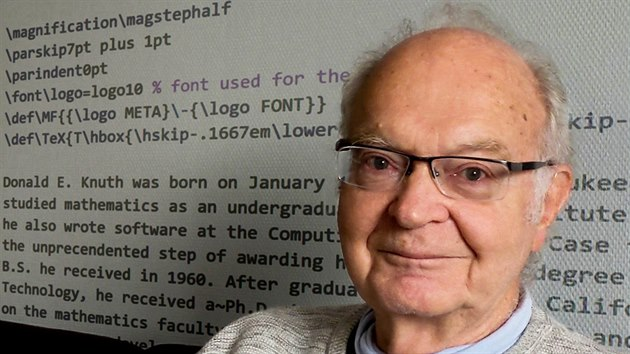
\includegraphics[scale=0.5]{pics/knuthi.jpg}
    \caption{Don Knuth -- CS Allfather}
    \label{fig:impl:knuth}
\end{figure}

Siehe und staune in Abb. \ref{fig:impl:knuth}.
\lipsum[6-9]
Dann betrachte den Code in Listing \ref{lst:impl:foo}.

\begin{lstlisting}[language=Python,caption=Some code,label=lst:impl:foo]
# Program to find the sum of all numbers stored in a list (the not-Pythonic-way)

# List of numbers
numbers = [6, 5, 3, 8, 4, 2, 5, 4, 11]

# variable to store the sum
sum = 0

# iterate over the list
for val in numbers:
    sum = sum+val

print("The sum is", sum)
\end{lstlisting}

\begin{spacing}{1}
\chapter{Zusammenfassung}
\end{spacing}



Mit dem vorgestellten Projekt Memoryland wurde bewiesen, dass ein immersives Erlebnis mit den Fotos erlebbar werden kann. Es wurden zwei Szenen als erste Beispiele in Unity umgesetzt. Die Waldszene soll die Erinnerung an Spaziergänge oder Wanderungen darstellbar machen. Die Inselszene hingegen, ermöglicht die Erinnerung an sonnige Urlaube an Sonne, Sand, Strand und Meer.

Viele weitere Szenen sind einfach umzusetzen und das Backend sowie das Frontend sind so umgesetzt, dass es einfach möglich ist diese zu integrieren. Es ist nahezu kein Aufwand (das Einfügen eines Datensatzes im Backend in der Memoryland-Type Tabelle) im Backend vonnöten und gar kein Aufwand in der Angular-Umsetzung des Frontend. Die Szenen selbst müssen in Unity entsprechend umgesetzt werden und dabei auf die Vorgaben für neue Szenen Rücksicht genommen werden.\footnote{siehe dazu Abschnitt \ref{subsec:unity-erweiterbarkeit}}

.......




\newpage
\pagenumbering{Roman}
\setcounter{page}{\value{RPages}}

\newacronym{guid}{GUID}{Globally Unique Identifier}
\newacronym{ide}{IDE}{Integrated Development Environment}
\newacronym{jit}{JIT}{Just In Time Compiler}
\newacronym{nfc}{NFC}{Near Field Communication}
\newacronym{rfid}{RFID}{Radio Frequency Identification}

% need : https://tex.stackexchange.com/a/536525

% Usage:
% \gls{label} lowercase in text
% \Gls{label} Uppercase in text
% \newacronym{label}{abbrev}{full}
% \newglossaryentry{label}{settings}



%\setlength{\glsdescwidth}{0.8\linewidth}
\glsnogroupskiptrue
\IfStrEq{\thesislang}{de}
{
	\printglossary[title=Glossar,toctitle=Glossar] %,style=long]
}
{
	\printglossary[title=Glossary,toctitle=Glossary] %,style=long]
}
\spacing{1}{
\IfStrEq{\thesislang}{de}
{
	\bibliographystyle{ieeetrande}
}
{
	\bibliographystyle{IEEEtran}
}
\bibliography{bib}
}
\listoffigures
\listoftables
\lstlistoflistings
\appendix
\addchap{Anhang}
\input{./sections/appendix}
\end{document}

